\section{Specifications}
\label{sec:specs}
\newcounter{SpecID}

\subsection{Markers}
\refstepcounter{SpecID}
\label{spec:markers}

The arena and tokens in the game are labelled with fiducial
markers. Each marker number is associated with a particular feature in the
arena, and also has an associated size. The marker numbers and sizes are as
follows:

\begin{center}
\begin{tabular}{lcc}
  \toprule
  \textbf{Item} & \textbf{Marker Number} & \textbf{Marker Size (\si{mm})} \\
  \midrule
  Arena boundary & 0 -- 27 & 250 \\
  Columns & 28 -- 43 & 250 \\
  Tokens belonging to the robot in zone 0 & 44 -- 49 & 100 \\
  Tokens belonging to the robot in zone 1 & 50 -- 54 & 100 \\
  Tokens belonging to the robot in zone 2 & 55 -- 59 & 100 \\
  Tokens belonging to the robot in zone 3 & 60 -- 63 & 100 \\
  % Robot Badges & 69 -- 73 & 100 \\
  \bottomrule
\end{tabular}
\end{center}

All markers are oriented vertically such that the human-readable text
is under the marker.

\subsection{Arena}
\refstepcounter{SpecID}
\label{spec:arena}

\begin{enumerate}
  \item The arena floor is an \SI{8}{m} $\times$ \SI{8}{m} square. The tolerance
        of these two dimensions is $\pm$\SI{250}{mm}.
  \item The floor of the arena is carpeted.
  \item The layout of the arena is given in \figref{fig:arena}.
  \item The outer walls of the arena are at least \SI{600}{mm} high, and the
        interior surface is white plastic-coated hardboard.
  \item Each wall of the arena features seven \SI{250}{mm} fiducial markers.
        The positions of these markers is given in \figref{fig:sidewall}.
        The marker numbering is given in \figref{fig:arena}.
  \item The robot starting zones are squares which share corners with the arena
        itself. Their sides are of length \si{1}{m}.
  \item Starting zones are numbered 0,1,2,3 clockwise starting at the north west corner.
  \item In the arena there are 4 fixed square columns with a height greater than
        or equal to \SI{370}{mm}, and a width of \SI{370}{mm}.
  \item Columns will have 4 different markers on each face, as given in
        \figref{fig:arena}.
  \item Markers will be placed on columns such that there is a \SI{120}{mm} 
        gap at the bottom.
  \item The scoring zones are squares of sides \si{2815}{mm}$\pm$\SI{50}{mm}
        positioned with the columns separating them.
  \item The starting and scoring zones is visually delineated on the floor of
        the arena by coloured tape. The outer edge of the tape indicates the
        outer edge of the zone. This tape is for visual reference only.
  \item \label{spec:tokenpos} Tokens will be placed in undisclosed layouts
        within an inner \si{2}{m} square of each scoring zone. The inner square
        is positioned such that two of its edges are the inside edges of the
        scoring zones. Tokens will start at least \si{150}{mm} from columns
        or other tokens and their layouts will be rotationally symmetric to
        that of other zones.
  \item Tokens will be placed in the scoring zone on the opposite side to their
        matching coloured scoring zone.
\end{enumerate}

\begin{sidewaysfigure}
  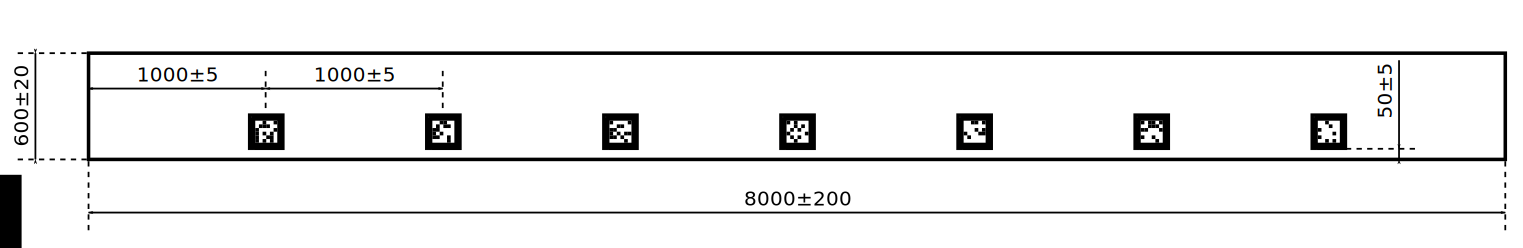
\includegraphics[scale=0.58]{fig-sidewall.pdf}
  \caption{Layout of markers along each arena wall.}
  \label{fig:sidewall}
\end{sidewaysfigure}

\begin{figure}
  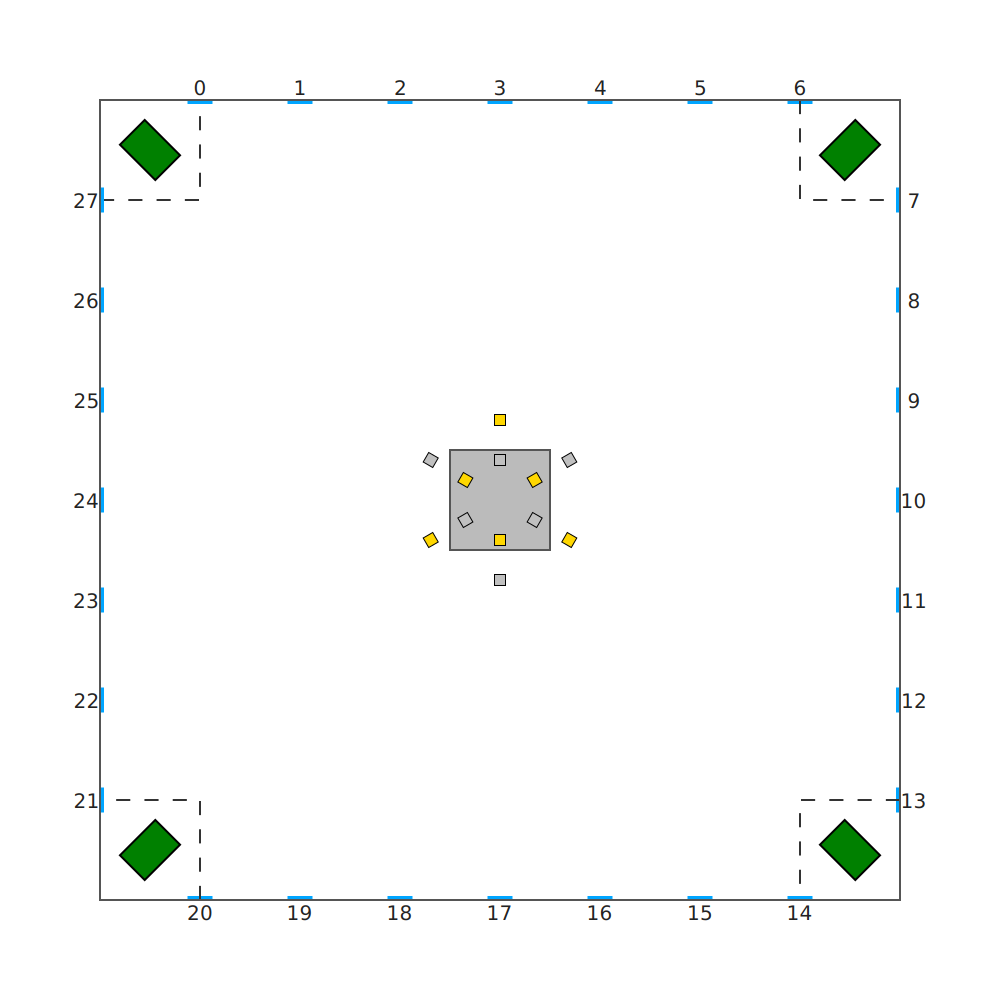
\includegraphics[scale=0.58]{fig-arena.pdf}
  \caption{Layout zones and tokens in the arena. Please note that tokens will
  be placed randomly but rotationally symmetrically within the respective
  scoring zones.}
  \label{fig:arena}
\end{figure}

\subsection{Tokens}
\refstepcounter{SpecID}
\label{spec:tokens}

\begin{enumerate}
  \item Tokens are cubic corrugated cardboard boxes, with sides of length
        \si{110}{mm}$\pm$\si{10}{mm}.
  \item Tokens will be coloured to match the colour of a scoring zone.
  \item Each face of each token has a fiducial marker attached.
  \item The initial layout of tokens in the arena is defined in
        \subspecref{spec:arena}{spec:tokenpos}.
\end{enumerate}
